\chapter{Entwicklung eines Qualitätssicherungsprozesses für agile Prozesse}
\label{cha:prozessentwicklung}

    Im Folgenden werden die Vor- und Nachteile der agilen Entwicklungsverfahren erarbeitet und miteinander verglichen. Daraus wird abgeleitet welche Kriterien für Softwarequalität mit agilen Prozessen verfolgt werden und für welche Charakteristiken ein Qualitätssicherungsansatz verfolgt werden muss. Daraufhin werden Möglichkeiten gezeigt, wie dieser Qualitätssicherungsansatz in die agile Methode einfließen kann.

    \section{Grenzen der agilen Entwicklung}

        Agile Vorgehensweisen lösen einige Probleme, sind aber keine universelle Lösung für Herausforderungen in Softwareprojekten. Vor jedem Projekt muss sich das verantwortliche Team Gedanken machen, ob eine agile Vorgehensweise angebracht und zielführend ist, oder ob zu konventionellen Methoden gegriffen werden sollte. Im Rahmen dieses Abschnitts soll eine Checkliste entwickelt werden, die dem verantwortlichem Team die Entscheidung erleichtern soll. Hierzu werden die Vor- und Nachteile der agilen Methoden gegenüber der traditionellen Softwareentwicklung im prozeduralen Ansatz betrachtet.

        Agile Entwicklungsmethoden sind mit dem Ziel entstanden schnell und kostengünstig auf geänderte Anforderungen zu reagieren, da die traditionelle Softwareentwicklung an einem strukturierten Planungsprozess mit anschließender Entwicklung und abschließendem Test festhält. Als erste These lässt sich daher ableiten, dass eine agile Methode angebracht ist, wenn die Anforderungen zu Beginn des Projektes nicht feststehen oder absehbar ist, dass sich diese während der Projektlaufzeit häufig ändern werden.
        Sollten die Anforderungen zu Beginn des Projektes feststehen und kann davon ausgegangen werden, dass sich diese im Rahmen des Projektes nicht verändern, sollte eine traditionelle Herangehensweise bevorzugt werden.

        Ein weiterer Vorteil von agilen Entwicklungsmethoden ist, dass im Rahmen einer Iteration stets ein lauffähiges Inkrement erstellt wird, dass potenziell an den Kunden ausgeliefert werden könnte. Dies erleichtert die Entscheidung das Projekt zu einem bestimmten Zeitpunkt oder bei Überschreiten eines bestimmten Budgets zu stoppen, da zu jedem Zeitpunkt ein fertiges Produkt besteht, dass die Funktionen mit der höchsten Priorität besitzt. Sollte das Projekt daher eine fixe Deadline oder einen engen Budgetrahmen haben, kann durch agile Entwicklungsmethoden die Wahrung dieser Vorgaben erleichtert werden.
        Wenn das Projekt jedoch sicherheitskritisch ist, exakter Spezifikation bedarf und umfangreiche Anforderungen hat, die erfüllt werden müssen, dann sollte sich an das Projekt eine lange und umfassende Testphase anschließen, um das Softwareprodukt zu validieren. So ist zum Beispiel bei Regierungsbehörden häufig die Funktionalität und Sicherheit höher gewichtet als das Budget und die Laufzeit. In diesem Fall ist ein traditioneller Ansatz angemessener, da sich die vollständige Erfüllung der Spezifikation bei einem umfassend geplanten Softwareprodukt leichter messen und überpüfen lässt als in einer Menge von Inkrementen.\footnote{Vgl. Leffingwell (High Assurance and Regulated Environments), S.2ff.}

        Wie in den vorherigen Kapiteln vorgestellt, ist es empfehlenswert, dass die Entwicklungsteams lokal zusammen arbeiten, um die Kommunikation und den Austausch zu fördern. Große räumliche Distanzen mindern die Effektivität der Methoden. Außerdem ist die Teamgröße bei etwa 12 Personen gedeckelt. Es gibt Fälle, in denen mehrere Scrumteams in einem großen Scrumteam organisiert sind und somit mehr Entwickler ein Projekt bearbeiten, aber der Verwaltungsaufwand wird hierdurch erhöht und die Produktivität vermindert. Agile Entwicklungsmethoden sind somit nur empfehlenswert, wenn eine überschaubare Anzahl an Entwicklern an einem Ort zusammenarbeit.
        Für sehr große Teams und verteilte Entwicklung ist ein hierarchischer, planender Ansatz besser geeignet.

        Durch die hierarchische Struktur in klassichen Projekten, bei der ein fester Plan von einer kleinen Menge kompetenter Personen in untere Hierarchiebenen durchgereicht wird, wird nur eine kleine Menge an sehr geschulten und fachlich versierten Mitarbeitern benötigt. Zur Ausführung eines konkreten Plans ist kaum Kreativität nötig. Scrum Teams dagegen planen ihre nächsten Schritte selbst und entwickeln in jeder Iteration ihren eigenen Plan. Um jedes Fachgebiet adäquat abgedeckt zu haben, werden kreativ denkende Kollegen verschiedener Fachrichtungen in einem Team gebündelt und organisieren sich selbst. Dadurch, dass Scrum-Teams ihre Ideen selbst umsetzen werden insgesamt mehr kompetente Personen benötigt, sobald die Organisation auf agile Entwicklungsmethoden setzt.\footnote{Vgl. Dombrowski (Lean Development), S.75ff.}
        Sollte eine hohe Anzahl an kompetenten Angestellten vorhanden sein, ist ein agiles Verfahren erfolgsversprechender.

        Ein letzter erfolgskritischer Punkt eines agilen Entwicklungsprojektes ist die ständige Verfügbarkeit eines Kunden, der die Entscheidungsgewalt hat, Vorgaben für das finale Produkt zu treffen. Sollte dieser nicht zur Verfügung stehen oder jegliche Entscheidungen in seinem Unternehmen abstimmen müssen, ist ein agiles Projekt gefährdet, da es ohne Kundenanforderungen keine Arbeitsgrundlage hat oder in Iterationen aufgehalten wird.

        \begin{table}
        \begin{tabularx}{\textwidth}{|X|c|c|}
          \hline
           & $\mbox{ }$Ja$\mbox{ }$ & Nein \\
          \hline
          Ständig wechselnde Anforderungen & $\Box$ & $\Box$ \\
          Feste Zeit-/Budgetvorgabe & $\Box$ & $\Box$ \\
          Lokale, kleine Entwicklungsteams & $\Box$ & $\Box$ \\
          Hohe Anzahl kompetenter Angestellter & $\Box$ & $\Box$ \\
          Ansprechpartner des Kunden & $\Box$ & $\Box$ \\
          \hline
        \end{tabularx}
        \caption{Checkliste zur Angemessenheit agiler Methoden}
        \label{tbl:checklist}
        \end{table}

        \autoref{tbl:checklist} fasst die oben erarbeiteten Ergebnisse zusammen. Sollte die Mehrheit der Punkte in der Tabelle \emph{Ja} anzeigen ist eine agile Entwicklungsmethode empfehlenswert. Andersherum verhält es sich genau gleich.

    \section{Vergleich der agilen Entwicklungsverfahren}

        Lean Software Development bildet für die Entwicklung einen Rahmen aus Prinzipien, die für jedes Projekt in Methoden und Anforderungen übersetzt werden müssen. Dies bietet zu Beginn eines Projektes die Freiheit das Rahmenwerk an die speziellen Anforderungen anzupassen. Wenn besonders umfangreiche Sicherheitsrichtlinien gesetzt werden, sind andere Methoden notwendig als bei einer möglichst schnellen Fertigstellung eines Produkts. Lean Software Development gibt dem Team die Möglichkeit ihren Methodensatz dahingehend anzupassen.

        Scrum setzt dagegen eine Managementmethodik fest, die die Kommunikation des Teams fördern und das Anforderungsmanagement optimieren soll. Durch eine Menge an vorher feststehenden Meetings und eines priorisierten Backlogs steht zu jedem Zeitpunkt fest, was im nächsten Sprint entwickelt wird. Die Sprints von vorher festgelegter Dauer minimieren den Stress der Entwickler, da sie sich nicht ständig an neue Anforderungen und Methoden gewöhnen müssen. Gleichzeitig bieten sie aber genügend Flexibilität, um auf den Kunden reagieren zu können.

        Extreme Programming verfolgt, wie der Name impliziert, einen sehr extremen Ansatz. Tests, Entwicklung und Flexibilität werden maximiert - teilweise zu Lasten der individuellen Freiheit. Durch einen sehr strikten Vorgehensansatz und festgelegte Methodiken, wird den Entwicklern Freiheit genommen mit dem Ziel die Ergebnisse zu optimieren. Extreme Programming trifft die Annahme, dass zu Beginn des Projektes nicht feststeht, wie das zu entwickelnde Produkt aussieht und daher die Anforderungen erst während der Projektlaufzeit festgehalten werden.

        Im Rahmen dieses Abschnitts werden die drei Vorgehensweisen verglichen. Die folgende Tabelle zeigt dabei die Ziele, Ansätze und Entwicklungsmethoden an:

        \begin{table}[H]
        \begin{tabularx}{\textwidth}{|p{2.5cm}|X|X|X|}
          \hline
            & Lean & Scrum & Extreme Programming \\
          \hline
          Ziele & Entscheidungen mit bestmöglichem Wissen treffen & Funktionen mit höchster Priorität erfüllen & Maximale Produktivität und Flexibilität
          \vspace{0.5\baselineskip} \\
          Ansatz & Ausprobierend, tastend & Dynamisch, Personenorientiert & Prozedural, Prozessorientiert
          \vspace{0.5\baselineskip} \\
          Entwicklungs-methode & Freie Methodenwahl & Freie Methodenwahl & Restriktiv, vorgeschrieben \\
          \hline
        \end{tabularx}
        \caption{Vergleich agiler Entwicklungsverfahren}
        \label{tbl:vergleich}
        \end{table}

        Wie in  \autoref{tbl:vergleich} zu sehen ist, hält das Extreme Programming mehr Restriktionen für die Entwickler bereit, während Scrum die Entscheidungsgewalt hinsichtlich der Methoden und Vorgehensweisen an das Scrum-Team weitergibt. Dadurch erhält ein Scrum-Team mehr Möglichkeiten aus den vergangenen Sprints zu lernen und Zeitpläne, Methodiken und Ziele im nächsten Sprint anders zu setzen. Wenn ein Extreme Programming Team dagegen feststellt, dass eine bestimmte User Story nicht umsetzbar ist, hat es keine Möglichkeit Einfluss auf die Methodik zu nehmen. Die Lean Software Development Vorgehensweise macht dagegen weder Vorgaben zur Entwicklung noch zum Management der Anforderungen und ist mit vorgegebenen Prinzipien die Allgemeinste der Methoden.

        Die Lean Methode kann durch Einsatz der Hilfsmittel aus Scrum und Extreme Programming ergänzt werden und nähert sich damit immer weiter den jeweiligen Methoden an. Aus den vorgegebenen Prinzipien zur Orientierung der Entwicklung wird dann eine Managementmethodik abgeleitet, die widerum zu einem ganzheitlichen Ansatz erweitert werden kann.

        Die agilen Vorgehensweisen lassen sich miteinander kombinieren, wobei eine sehr abstrakte Methode sich einer sehr konkreten Methode annähert, je mehr Werkzeuge sie dieser entnimmt.

        Da alle agile Methoden auf dem agilen Manifest beruhen, haben sie in ihren Kernannahmen viele Gemeinsamkeiten. Alle Methoden nehmen an, dass die Anforderungen an das Produkt zu Beginn der Entwicklung nicht feststehen und wollen somit möglichst flexibel auf Änderungen reagieren. Beim Lean Software Development wird es durch mehrere konkurrierende Entwürfe realisiert, die auf Grundlage einer, im laufenden Projekt erweiterten Faktenbasis. gefiltert werden, bis eine Entscheidung getroffen werden kann. Scrum und Extreme Programming setzen dagegen auf Iterationen, die die am höchsten priorisierten Wünsche des Kunden umsetzen und sich so dem Soll-Ergebnis annähern.

        Gemeinsam ist den Methoden außerdem, dass sie die Entwickler in den Mittelpunkt rücken. Alle agilen Methoden geben den Entwicklern einen Vertrauensvorschuss und erwarten Kreativität und Fachkenntnisse bei der Lösung. Im Gegensatz zu herkömmlichen Methoden wird der Plan und die Umsetzung von den ausführenden Personen beschlossen und nicht von einer kleinen Menge ranghöherer Angestellter.

        Unterschiede zwischen den Methoden sind darin begründet, dass sie an verschiedenen Ebenen ansetzen. Lean lässt sich auch auf Wasserfallmodelle anwenden und nicht nur auf iterative Methoden, da es nur Prinzipien vorgibt, an denen sich orientiert werden soll. Scrum gilt als Managementprozess, der die Entwicklung offen lässt. Extreme Programming ist allumfassend aufgesetzt.

        \begin{figure}[!htbp]
            \begin{center}
                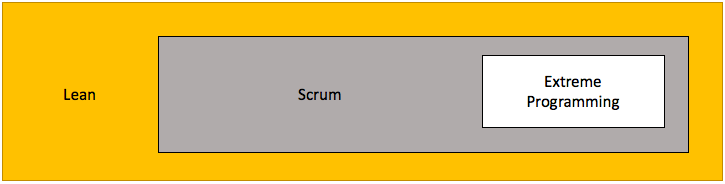
\includegraphics[width=11cm]{Abbildungen/ag_methoden}
                \caption[Umfang agiler Methoden im Vergleich]{Umfang agiler Methoden im Vergleich}
                \label{abb:vergleich}
            \end{center}
        \end{figure}

        \autoref{abb:vergleich} illustriert nochmals das Verhältnis der Verfahren. Je mehr Werkzeuge einer inneren Methode gewählt werden, desto mehr nähert sich das Verfahren dem Extreme Programming an. Da in dieser Arbeit agile, iterative Methoden betrachtet werden sollen, werden die Qualitätssicherungsmethoden auf die Scrum Vorgehensweise angewandt, da diese die am weitesten gefasste Methode ist, die Iterationen vorsieht. Die Methoden des Extreme Programmings und Prinzipien des Lean Software Developments werden, wenn nötig und angemessen, ergänzend hinzugezogen.

        Zu beachten ist, dass sich die in dieser Arbeit betrachteten Methoden nicht widersprechen. Die Prinzipien des einen Modells werden beispielsweise durch Methoden des Anderen umgesetzt. Im Folgenden wird die Scrum Methodik als Basis des Prozesses genutzt, falls es jedoch der Qualität zu Gute kommt, um Methoden des Extreme Programming oder Lean Software Developments ergänzt. Außerdem ist Scrum der in der SAP SE verwendete Ansatz agiler Entwicklungsmethoden.

    \section{Qualität durch agile Methoden}

        Dieses Kapitel zeigt, welche Qualitätsstandards für Software durch die Anwendung der agilen Methoden bereits erfüllt werden. Im Anschluss wird geprüft, wie die agilen Methoden durch Qualitätssicherungsmodelle ergänzt werden können, um eine umfangreiche und zufriedenstellende Softwarequalität zu gewährleisten.

        Wie im Grundlagenteil bereits erläutert wird sollte besonders viel wert darauf gelegt werden, dass eine Software funktional, verlässlich und wartbar ist.

        \subsection{Funktionalität}

            Funktionalität wird daran gemessen, dass Software die geforderten Funktionen sicher, genau und in Zusammenarbeit mit anderen Systemen erfüllt. Scrum liefert mit jedem Sprint eine potenziell auslieferbare Software, die vom Kunden bewertet wird, um die Richtung des Projektes zu steuern. Die am höchsten priorisierte, noch nicht realisierte Funktion wird dabei stets als das Ziel des nächsten Sprints definiert. Somit wird in den ersten Sprints eine Basisfunktionalität geliefert, die ständig erweitert wird. Das Projekt kann beendet werden, sobald alle Anforderungen an die Funktionalität erfüllt sind. Agile Methoden liefern somit ein wichtiges Fundament zur Erstellung von funktionaler Software. Im Gegensatz zu klassischen Methoden der Softwareentwicklung kann der Kunde die Software am Ende des Projektes in jedem Fall einsetzen und müsste bei vorzeitigem Projektende lediglich mit einem reduzierten Funktionsumfang auskommen. Die Passgenauigkeit (\emph{Suitability}) ist also sehr hoch.

            Um die Akkuranz (\emph{Accuracy}) der Software zu gewährleisten muss sie stets die erwarteten Resultate und Effekte erzielen, die sich der Anwender von der Funktion erhofft. In der Scrum-Entwicklung werden die erwarteten Effekte vom Product Owner dargestellt und vom Team ausgearbeitet. Hier erscheint es vorteilhaft die User-Stories und Unit-Tests des Extreme Programming zu verwenden. Der Anwender beschreibt seine Aufgabe, seine Eingaben in die Software und die erwartete Ausgabe. Diese werden in Unit-Tests umgesetzt und ein erfüllter Unit-Test entspricht bei konsequenter Umsetzung einer Rückgabe der erwarteten Resultate. Auch die Akkuranz lässt sich durch den Einsatz agiler Methoden sicherstellen.

            Die Zusammenarbeit mit anderen Systemen (\emph{Interoperability}) ist abhängig von der umliegenden Architektur. Im Falle von einer serviceorientierten Architektur können sehr gut Datenflüsse zwischen den Systemen simuliert werden, um so User-Stories und Unit-Tests zu erfüllen. Bei einer direkten Anbindung an historisch gewachsene Altsysteme, die beispielsweise zum Reporting für Kennzahlen dienen, erweist sich der Test schwerer, da diese in der Entwicklungsumgebung meist nicht zur Verfügung stehen. Die Kommunikation an Schnittstellen muss daher vor Beginn der Entwicklung eines Moduls spezifiziert werden. Ein umfangreicher Test eben dieser kann erst bei der Integration in die Landschaft des Kunden erfolgen. Hier sollten weitere Qualitätssichernde Maßnahmen gestartet werden.

            Zuletzt ist im Rahmen der Funktionalität die Sicherheit (\emph{Security}) zu beachten. Es ist sicherzustellen, dass unauthorisierte Personen und Systeme keinen Zugriff und authorisierte Nutzer und Systeme Zugriff auf die betreffenden Systeme haben. Wie in ISO 9126-1 als Notiz angemerkt ist Sicherheit \enquote{a characteristic of quality in use, as it does not relate to software alone, but to a whole system.}\footnote{ISO 9126-1 (Information Technology), S.8} Die Software kann nicht am Ende eines Sprints auf Sicherheit geprüft werden. Um die Sicherheit zu garantieren, muss das vollständig auslieferbare Produkt zuzüglich aller Schnittstellen zu Umsystemen geprüft werden. Dies kann ebenfalls nicht im Rahmen eines agilen Prozesses ablaufen.

            Für die Funktionalität bedeutet dies, dass agile Prozesse die gewünschten Funktionen und Ausgaben produzieren, aber die Zusammenarbeit mit umliegenden Systemen und die Sicherheit des gesamten Systems separat geprüft und sichergestellt werden sollte.

        \subsection{Verlässlichkeit}

            Bei Unternehmen der Finanzdienstleistungsbranche ist es unerlässlich, dass Software stets wie erwartet reagiert und ungültige Eingaben herausfiltert, da Fehler in der Software die Kundenzufriedenheit, und somit auch das Kundenvertrauen, senken können und bei Berechnungen von beispielsweise Kontoständen auch Rundungsfehler sehr große Abweichungen nach sich ziehen. Unit-Tests vergleichen die Resultate der Software mit erwarteten Ergebnissen und geben auf Grund dieses Vergleiches einen erfolgreichen Test zurück oder einen Fehler. Somit wird zumindest auf erwartete Ergebnisse geprüft.

             Abgesehen von der Richtigkeit produzierter Ergebnisse, muss auch überprüft werden, ob das Produkt allgemein keine Fehler auf Grundlage von Fehlern im Programm wirft. Die Reife (\emph{Maturity}) eines Softwareproduktes wird daran gemessen, dass der Programmablauf in sich fehlerfrei ist. Ein Scrum-Team testet sehr viel und durchläuft die Software durch automatisierte Tests sehr häufig, bevor es diese zum Kunden ausliefert. Durch viele automatisierte Tests sollten alle Fehler der Software noch während der Entwicklung zum Vorschein kommen und eliminiert werden können. Fehler in der Software werden somit schon während der Entwicklung abgefangen.

            Die Fehlertoleranz (\emph{Fault tolerance}) einer Software gibt an, wie sehr sie von ungültigen Eingaben, falscher Kommunikation von Seiten der Schnittstellen und Hardwarefehlern abhängig ist. Das Ziel der Software sollte es sein Fehler zu entdecken und zu melden, um die Vermeidung, beziehungsweise Korrektur, eben dieser zu erleichtern. Ein Ausfall der Hardware kann von Seiten der Entwickler nicht verhindert werden. Die Sicherheitsmaßnahmen gegen Hardwaredefekte werden im nächsten Absatz behandelt. Empfohlen werden lediglich redundante Hardwarekomponenten, sodass kein Single-Point-of-Failure existiert. Falsche Kommunikation der Schnittstellen kann ebenfalls nicht durch das Scrum-Team verhindert werden, da dieses die Schnittstellen nicht vor Ort testen kann um mögliche Fehler auszuprobieren. Die Prüfung von Schnittstellen und Hardware sollte somit im Rahmen eines umfassenden Integrationstest stattfinden.
            Falsche Benutzereingaben lassen sich bereits während des Tests abfangen, indem eine Prüfung die Eingaben validiert und mit erwarteten Eingaben vergleicht. Hier werden neben den automatisierten Tests umfassende Gültigkeitstests benötigt.
            Die Reaktion der Software auf fehlerhafte Eingaben sollte am Ende der Entwicklung umfangreich getestet werden.

            Zuletzt sollte bei einem Defekt ein sicherer und korrekter Zustand des Systems möglichst schnell wiederhergestellt (\emph{Recoverability}) werden. Dies setzt regelmäßige Back-Ups und eine redundante Datenhaltung voraus. Während der Entwicklung sollte daher geprüft werden, wie sich die Software verhält, wenn sie unerwartet unterbrochen wird, beispielsweise durch einen Stromausfall. Die häufigsten und bekanntesten Ausfallszenarien von Software, wie Netzwerkfehler, menschliche Fehler, Stromaufall und Wetterunfälle\footnote{Vgl. Statista (Ursachen von IT-Ausfällen).} lassen sich sehr gut replizieren, testen und daher abfangen. Sie sollten daher in produktiver Software nicht vorgefunden werden.

            Die Verlässlichkeit der Software im Hinblick auf ungültige Eingaben sollte vor Produktivsetzung geprüft werden. Die Wiederherstellbarkeit und Reife der Software lassen sich jedoch in der Entwicklungsumgebung sicherstellen.

        \subsection{Wartbarkeit}

            Extreme Programming empfiehlt bei der Entwicklung der Software keine zukünftigen Erweiterungen im Code zu ermöglichen. Dies geschieht unter der Annahme, dass eine einfach gehaltene Software ohne überflüssigen Code leichter zu erweitern ist, als eine umfangreiche Software, die speziell auf Erweiterungen ausgelegt ist, die vielleicht nie genutzt werden. Der inkrementelle Ansatz von Scrum und Extreme Programming bedeutet, dass eine Vielzahl an Bausteinen entsteht, die miteinander und in das bestehende System integriert werden. Wenn ein neues System an einen bestimmten Baustein angeschlossen werden muss, kann es sein, dass daher nur ein Glied dieser modularen Systemkette verändert werden muss, statt ein umfassendes System.

            Als erster Teil der Wartung wird vorgesehen, dass das bestehende System analyisiert (\emph{Analyzability}) werden kann. Dies bedeutet, dass der Code auf Fehler untersucht wird, oder geprüft wird, ob Veränderungen notwendig sind. Ein Vorteil der agilen Vorgehensweisen ist, dass die Dokumenation direkt im Code stattfindet und somit keine veralteten Dokumente als Grundlage dieser Analyse dienen. Im Extreme Programming gehört der Code zudem allen Entwicklern. Somit ist es möglich, dass mindestens ein Entwickler verfügbar ist, der Fragen beantworten kann. Die Verständlichkeit und analysierbarkeit des Codes ist bei konsequenter Umsetzung der agilen Prinzipien sehr hoch.

            Während der agilen Entwicklung und insbesondere beim Extreme Programming wird der Code ständig neu strukturiert beziehungsweise Refactored. Die Gliederung des Hauptprogramms in eine Menge von Methodenaufrufe erleichtert es, Teile der Software zu verändern (\emph{Changeability}). Die Modularisierung der Software in wiederverwendbare Methoden erleichtert zudem die Korrektur von Fehlern, da diese nur an einer Stelle stattfinden muss. Der Code ist darauf ausgelegt ständigen Veränderungen unterworfen zu sein. Hiermit ist auch die Veränderbarkeit in einem agil entwickelten Softwareprodukt gegeben.

            Im Rahmen von Unit-Tests kann überpüft werden, ob sich das Verhalten der Software auf Grund von Änderungen im Code geändert hat. Sollten diese Unit-Tests nach einer Veränderung keine korrekten Ergebnisse liefern muss der Code weiter angepasst und der Fehler gesucht werden. Die Stabilität (\emph{Stability}) der Software, dass heißt, die Fähigkeit unerwartete Effekte von Veränderungen zu verhindern, ist sehr hoch.

            Zuletzt ist gefordert, dass veränderte Software validiert werden kann (\emph{Testability}). Eine Softwarevalidation ist der \enquote{Prozess des Bestätigens, dass die Spezifikation einer Phase oder des Gesamtsystems passend zu oder konsistent mit den Anforderungen des Kunden ist.}\footnote{Bresser (Validierung und Verifikation).} Die Software wurde zusammen mit einem Kunden auf Grundlage von direkter Kommunikation und, falls angewandt, User-Stories und Unit-Tests entwickelt. Ein Vergleich mit einer Spezifikation ist nicht möglich, da diese nicht angelegt ist. Um, wie von den agilen Prinzipien vorgeschrieben, keine allzu umfassende Dokumentation der Anforderungen anfertigen zu müssen, ist es empfehlenswert die Validierung der Anforderungen anhand von existierenden Dokumenten zu erledigen. Die Anforderungen des Kunden werden vom Product Owner im Backlog zusammengefasst und auf Grundlage dieses Backlogs werden die Funktionen, die die Software besitzen soll, priorisiert und in das Entwicklungsteam hereingetragen. Der Backlog stellt somit alle Anforderungen dar, die der Kunde gestellt hat. Am Ende jedes Sprints wird das fertige Inkrement dem Kunden vorgestellt und dieser gibt sein Feedback dazu ab. Wie zuvor beschrieben muss bei der Anfertigung des Backlogs ein klares Bild beim Entwicklungsteam und beim Kunden bestehen, was als Definition von \emph{Done} festgelegt ist. Gibt der Kunde daher nach einem Sprint sein \emph{Done} zu einem Produkt, kann es im Backlog als erledigt markiert werden. Um am Ende die Anforderungserfüllung zu überprüfen, muss nur der Backlog vorgelegt werden.

            Zusammenfassend lässt sich sagen, dass die Wartbarkeit des Codes und des Softwareproduktes allgemein durch agile Methoden deutlich erleichtert wird. Der modulare Aufbau des Systems ermöglicht zudem die Integration und Einbindung von neuen Systemen.

    \section{Qualitätssichernde Erweiterung der agilen Methoden}

        %Zunächst werden die Punkte notiert, wo zusätzliche QUalitätssicherung von Nöten ist. An dieser Stelle wird erklärt wie es bei der herkömmlichen Softwareentwicklung gelöst wird und welche Methoden der Qualitätssicherung, bpsw. des Testens angewandt werden können. Wenn alle groben Probleme abgedeckt sind kann man sich an Null-Fehler / Dokumentation wie in ISO 9000 gefordert verrennen.

        Wie im letzten Abschnitt erarbeitet sollten folgende Punkte durch zusätzliche Qualitätssicherungsmethoden ergänzt werden, um auch in agilen Projekten Qualität sicherzustellen.

        \begin{itemize}
          \item Functionality
            \begin{itemize}
              \item Interoperability
              \item Security
            \end{itemize}
          \item Reliability
            \begin{itemize}
              \item Fault Tolerance
            \end{itemize}
          \item Maintainability
        \end{itemize}

        In \autoref{subsec:kritchar} werden die kritischen Sub-Charakteristiken beleuchtet und beispielhaft Vorgehensweisen der Qualitätssicherung und der klassischen Softwareentwicklung vorgestellt, die den unsicheren Ergebnissen der agilen Entwicklung entgegen wirken.

        \subsection{Kritische Charakteristiken}
        \label{subsec:kritchar}

            \subsubsection{Interoperabilität}

                Um die Interoperabilität der Software mit den umliegenden Systemen zu gewährleisten, müssen die Schnittstellen spezifiert werden. Eine Herausforderung, die bei der agilen Entwicklung besteht ist, dass die Software in enger Zusammenarbeit mit genau einem Kunden entwickelt wird, um diese genau auf seine Wünsche zuzuschneiden. Da die SAP SE ein Anbieter von Standardsoftware und kein Anbieter von Individualsoftware ist, muss die Software nach Fertigstellung bei einem Referenzkunden generalisierbar sein, um relevant zu bleiben.

                \begin{table}[H]
                    \begin{tabularx}{\textwidth}{|X|X|}
                        \hline
                        Herausforderung & Lösungsansatz \\
                        \hline
                        Kommunikation mit umliegenden Systemen & Schnittstellenlandkarte zu Beginn des Projekts erarbeiten \\
                        \vspace{0.5\baselineskip}
                        Wiederverwendbare Schnittstellen & \vspace{0.5\baselineskip} Verwendung anerkannter Standards zur Interoperabilität (Web-Services) \\
                        & Dokumentation der entwickelten Schnittstellen \\
                        \hline
                    \end{tabularx}
                    \caption{Lösungsansatz zur Interoperabilität}
                \end{table}

                Bei einem klassischen Softwareprojekt im Rahmen der Accelerated SAP Methodik wird zu Beginn des Projektes eine Service- und Schnittstellenlandkarte erstellt, die alle bestehenden Systemen auflistet und zeigt, welche Schnittstellen in der neuen Software benötigt werden.
                Dies ist eine manuelle Aufgabe, die von Experten des Systems in Zusammenarbeit mit SAP Experten ausgearbeitet wird. Es werden alle Systeme aufgelistet und auf Grundlage dieser die Schnittstellen von und zu diesen dokumentiert. Dabei wird notiert wer eine Schnittstelle wann benutzt. Mit diesem System- und Schnittstellendokument kann das Scrum-Team die Software aufbauen und mit Testdaten befüllen. Im Idealfall wird eine technologieunabhängige Kommunikation etabliert, beispielsweise über Web-Services.

                \begin{quote}
                    \enquote{Companies that regularly hand off data between systems such as those in the financial services, energy trading, high-tech manufacturing, and telecommunications industries are ideal candidates for Web services technologies.}\footnote{Chung (Web Services Computing), S.36.}
                \end{quote}

                Genau spezifizierte Schnittstellen auf Grundlage von Web-Services bieten den Vorteil, dass die Datentypen unabhängig von Anfragenden und Antwortenden sind, indem die Nachrichten über einen Enterprise Service Bus geroutet und von ihm übersetzt werden. Mit der Einführung einer Orchestrierungsebene bei jeder neuen Softwareeinführung ist die Implementierung des Scrum-Teams technologie-, system- und kundenunabhängig und eine, in diesem Fall auch außerhalb des Quellcodes gut dokumentierte Anforderung an Services, genügt für eine Integration.

                Das Ergebnis einer solchen, konsequent umgesetzten Vorgehensweise, ist eine modulare, serviceorientierte Architektur. Durch dies können einzelne Komponenten ersetzt werden, sobald das jeweilige Modul im Rahmen eines Sprints fertig gestellt ist. Die Funktionalität jeder Komponente kann daher in einer produktiven Umgebung getestet werden, indem ein neues Modul ohne tatsächliche Verantwortung, Daten bezieht und wieder zurück gibt. Diese können dann mit der bestehenden Software oder den erwarteten Ausgaben verglichen werden kann.

                Um Interoperabilität, wie im oben aufgeführten Beispiel, zu erreichen, sollte das Scrum-Team mit Hilfe eines Referenzkunden eine standardisierte, technologieunabhängige Kommunikation anstreben, die, außerhalb des Codes, verständlich dokumentiert wird. Eine Verwendung von anerkannten Standards wird ebenfalls im Rahmen der ISO 9126-1 empfohlen.\footnote{Vgl. ISO 9126-1 (Information Technology), S.9.}

            \subsubsection{Sicherheit}

                Die Sicherheit von Software kann auf zwei Wegen gewährleistet werden. Durch eine Verifikation und Validierung werden Fehler aufgedeckt, die im Rahmen der Entwicklung entstanden sind und durch nachträgliche Korrektur eliminiert werden können. Die zweite Vorgehensweise ist die Software Security Assurance, die Fehler während der Entwicklung vermeiden soll. Konform zum Six Sigma Prinzip, dass fehlerfreie Prozesse als Grundlage für fehlerfreie Resultate sieht, sollte die Ursache bekämpft werden statt nachzubessern. Der Fokus während der Entwicklung sollte daher auf die Software Security Assurance gelegt werden. Eine nachträgliche Prüfung ist dennoch empfohlen. Ein verantwortungsvoller Umgang der Anwender der Software wird vorausgesetzt, da das Scrum-Team keinen Einfluss auf die Mitarbeiter des Unternehmens nehmen kann.

                \begin{table}[H]
                    \begin{tabularx}{\textwidth}{|X|X|}
                        \hline
                        Herausforderung & Lösungsansatz \\
                        \hline
                        Sicherheitsfehler vermeiden & Aufnahme von Sicherheitsexperten im Entwicklerteam \\
                        & Sichere, verifizierte Standards verwenden \\
                        & Vorschriften der bestehenden Software beachten \\
                        & Doppelte Kontrolle durch Pair Programming \\
                        & Sicherheit als User-Story \\
                        \vspace{0.5\baselineskip} Sicherheit überprüfen & \vspace{0.5\baselineskip} Sicherheit dokumentieren \\
                        & Umfangreiche Systemtests nach Vollendung des Projekts \\
                        & Formale Validierung und Verifikation \\
                        \hline
                    \end{tabularx}
                    \caption{Lösungsansatz zur Sicherheit}
                \end{table}

                Sicherheit kann, und muss, auf der System- und der Softwareebene sichergestellt werden. Die Systemebene setzt hauptsächlich auf Verschlüsselung und Zugriffskontrollen, während die Softwarebene ausnutzbare Lücken im Quelltext vermeiden soll.

                Maßnahmen auf der Systemebene umfassen unter anderem Firewalls, Daten- und Netzwerkverschlüsselung, Zugriffskontrollen und Authorisierungs- bzw. Authentifizierungsmechanismen. Die Sicherheit auf Systemebene muss nach Fertigstellung der einzelnen Softwarekomponenten entwickelt werden und allumfassend sein.\footnote{Vgl. Goertzel (Enhancing the development life cycle), S.6.}
                Für die Iterationen sollte nur Wert auf eine sichere Kommunikation zwischen den Modulen des Systems gelegt werden. Diese sollte durch die oben genannten Kommunikationsstandards gewährleistet sein. Wenn Vorschriften und Sicherheitsmerkmale in dem System bestehen, in das die Software eingebettet werden soll, dann müssen diese an das Scrum-Team herangetragen werden und in der Entwicklung beachtet werden.

                Angreifbare Schwachstellen in der Software zu vermeiden ist die Aufgabe des Scrum-Teams. Zur Vermeidung von offensichtlichen Mängeln kann die Extreme Programming Technik des Pair Programmings angewandt werden. Durch zwei Entwickler, die den Quellcode kontrollieren, und ständig überprüfen, kann eine erste Menge von Mängeln abgefangen werden. Die Aufmerksamkeitsspanne von zwei Personen ist größer und somit werden Flüchtigkeitsfehler unterbunden.

                Um weitere Fehler zu vermeiden, und die Sicherheit der Software zu garantieren, wird eine umfangreiche Dokumentation vorausgesetzt. Die Dokumentation einer sich ständig verändernden Software ist ein umfangreiches und zeitintensives Projekt, sodass effizientere Methoden gefunden werden müssen. Eine Möglichkeit, um die Sicherheit der Software in den Rahmen eines agilen Projektes einzugliedern ist die Sicherheit als User-Story.\footnote{Vgl. Wäyrynen (Security Engineering), S.11.} Dies kann dabei eine klassische User-Story sein, wie zum Beispiel: \emph{Als Anwender möchte ich eine Software verwenden, die unzulässige Eingaben von mir abfängt und keinen unabsichtlichen oder absichtlichen Schaden durch meine Interaktion zulässt}. Eine andere Möglichkeit sind Misuse-Stories, die schädliches Verhalten eines Anwenders simulieren und abfangen müssen.

                Ergänzend kann die Aufnahme eines Sicherheitsexperten in das Entwicklerteam die allgemeine Aufmerksamkeit gegenüber der Sicherheit erhöhen und ist daher auch empfehlenswert.

            \subsubsection{Fehlertoleranz}

                Vor der Fehlertoleranz von Software steht die Fehlervermeidung. Jeder Fehler, der während der Entwicklung abgefangen wird, muss nicht während der Laufzeit des Programms behandelt werden. Hierfür bieten die agilen Verfahren, die auf Grundlage des Test-Driven Developments arbeiten, sehr gute Methoden durch automatisierte Tests, die sehr häufig laufen und die meisten Erwartungswerte abdecken. Automatisierte Tests sind meistens Black-Box Tests, die das Ergebnis eines Methodenaufrufs mit erwarteten Ergebnissen vergleichen. Im Rahmen eines Black-Box Tests müssen alle möglichen Eingaben eines Anwenders abgedeckt werden. So müssen auch ungültige Eingaben getätigt werden, um zu prüfen, ob diese erfolgreich abgefangen werden.
                Eine weitere Möglichkeit neben dem Black-Box Test bietet der in \autoref{subsec:analytischeqs} vorgestellte Strukturtest einer Software. Dieser ist durch Unit-Tests nicht abgedeckt und nur das Pairprogramming bietet eine Annäherung zum White-Box Test. Eine Durchführung von Strukturtests während der Entwicklung sollte in regelmäßigen Abständen stattfinden, beispielsweise am Ende jeder Woche.
                Eine Kombination dieser beiden Tests führt dazu, dass Mängel der Ergebnisberechnung und Mängel des Codes weitgehend eliminiert werden.

                \begin{table}[H]
                    \begin{tabularx}{\textwidth}{|X|X|}
                        \hline
                        Herausforderung & Lösungsansatz \\
                        \hline
                        Vermeidung von Softwarefehlern & Unit-Tests (Test-Driven Development) \\
                        & Regelmäßige Strukturtests \\
                        \vspace{0.5\baselineskip} Toleranz gegenüber Softwarefehlern & \vspace{0.5\baselineskip} Redundantes Auführen von Operationen \\
                        & Unabhängige, konkurrierende Algorithmen implementieren \\
                        \vspace{0.5\baselineskip} Missbrauch von Schnittstellen verhindern & \vspace{0.5\baselineskip} Kommunikation von und zur Softwarekomponente spezifieren \\
                        & Verwenden von Kommunikationsstandards \\
                        \hline
                    \end{tabularx}
                    \caption{Lösungsansatz zur Fehlertoleranz}
                \end{table}

                Die Möglichkeit, dass der Code Lücken enthält oder nicht alle Sonderfälle abgedeckt sind, besteht trotz der beiden Testverfahren. In diesen Fällen muss die Fehlertoleranz verhindern, dass der Anwender falsche, ungültige oder keine Ergebnisse erhält.

                Um die Sicherheit und Ausfallwahrscheinlichkeit von Hardware zu minimieren, werden alle Module redundant installiert, sodass der Ausfall eines Teils nicht das System zum Einsturz bringt. Genau wie bei Hardware kann es auch bei Software hilfreich sein redundante Operationen laufen zu lassen. Software ist im Gegensatz zu Hardware von zufälligen Ausfällen unabhängig und reagiert auf die gleiche Eingabe mit der gleichen Ausgabe.\footnote{Vgl. Chen (N-Version Programming), S.113.} Es kann dennoch vorteilhaft sein ein Programm zur gleichen Zeit mehrfach zu starten und die Ergebnisse zu vergleichen, da Servereingaben oder Informationen aus anderen Systemen unvollständig ankommen könnten oder, bei Thread-basierten Systemen, Schreib- und Leseprozesse blockiert werden könnten, was bei manchen Anwendungsfällen nicht auffällt. Damit die konkurrierenden Prozesse absolut unabhängig voneinander arbeiten, müssen sie individuell implementiert sein und auf eigenen Datenbasen arbeiten. Je mehr Prozesse gleichzeitig redundant ablaufen, desto höher ist die Wahrscheinlichkeit das korrekte Ergebnis zu erhalten.

                Ergänzend hierzu kann die selbe User-Story mit verschiedenen Algorithmen umgesetzt werden. Dies erfordert zwar den doppelten Code-Aufwand, da die beiden Lösungen absolut unabhängig sein sollen, erhöht aber weiterhin die Fehlertoleranz. Die Entwicklung von konkurrierenden, unabhängigen Algorithmen sollte daher nur bei höchst kritischen Projekten angewandt werden.
                Probleme aufgrund von Softwarefehlern werden durch oben genannte Methoden auch in agilen Projekten weitestgehend eliminiert.

                Um zu gewährleisten, dass das Programm durch vorsätzlichen Missbrauch von Schnittstellen nicht angegriffen wird, sollte die Kommunikation von und zur Software spezifiziert werden. Hier bieten sich die zuvor erwähnten Web-Services an, die eine standardisierte Anfrage an die Software zulassen und eine Antwort festlegen. So kann sich das angesprochene System und das anfragende System sicher sein, gültige und valide Daten zu erhalten. Software, die mit Anwendereingaben arbeitet, kann ähnlich vorgehen, da die Anfragen bei der häufig verwendeten 3-Schichten-Architektur ebenfalls von außen an das System herangetragen werden.

                Um die Fehlertoleranz einer Software sicherzustellen, sollten daher zunächst präventive Maßnahmen ergriffen werden, da ein Fehler nie vollständig umgangen werden kann. Konventionen und Standards helfen jedoch dabei möglichst wenig Fehler zu machen, da diese durch eine Vielzahl von Personen geprüft und getestet wurden und somit die höchste Zuverlässigkeit bieten - insbesondere bei der Kommunikation zwischen Modulen und Systemen. Für die Kommunikation zwischen Finanzanwendungen hat das Banking Industry Architecture Network zudem ein Rahmenwerk veröffentlicht, dass neben einheitlichen Kommunikationsstandards ein einheitliches Datenmodell vorgibt. Somit kann auch die Art der zu übertragenden Arten genau spezifiziert werden. 